%%%%%%%%%%%%%%%%%%%%%%%%%%%%%%%%%%%%%%%%%%%%%%%%%%%%%%%%%%%%%%%%%%%%%%%%
% Plantilla TFG/TFM
% Escuela Politécnica Superior de la Universidad de Alicante
% Realizado por: Jose Manuel Requena Plens
% Contacto: info@jmrplens.com / Telegram:@jmrplens
%%%%%%%%%%%%%%%%%%%%%%%%%%%%%%%%%%%%%%%%%%%%%%%%%%%%%%%%%%%%%%%%%%%%%%%%

\chapter{Pruebas}

En este capítulo se describen las pruebas realizadas sobre el sistema desarrollado con el objetivo de verificar su correcto funcionamiento desde un punto de vista funcional y de usuario. Las pruebas se han centrado en validar el comportamiento del sistema de extremo a extremo, comprobando la correcta integración entre el frontend web, el backend y los dispositivos de red monitorizados.

No se han realizado pruebas unitarias ni de rendimiento específicas, ya que el objetivo principal de este trabajo es demostrar la viabilidad y funcionalidad del sistema como herramienta de monitorización y gestión de red. Las pruebas presentadas a continuación constituyen una evidencia clara de que el sistema responde adecuadamente ante los escenarios de uso previstos.

\section{Entorno de pruebas}

Las pruebas se han llevado a cabo en un entorno controlado compuesto por routers Cisco simulado mediante GNS3, una máquina virtual con sistema operativo Linux encargada de ejecutar el backend y el frontend web, y un navegador web desde el que se accede a la aplicación. Este entorno permite reproducir de forma realista el comportamiento de una red de comunicaciones y validar las funcionalidades implementadas sin necesidad de disponer de equipamiento físico.

\section{Pruebas de funcionalidad end-to-end}

En esta sección se presentan las principales pruebas funcionales realizadas, abarcando el flujo completo de operación del sistema, desde la interacción del usuario hasta la comunicación con los dispositivos de red y la visualización de resultados.

\subsection{Prueba de autenticación de usuario}

La primera prueba consiste en verficar el acceso al sistema mediante autenticación de usuario. Para ello, el usuario introduce sus credenciales en la pantalla de inicio de sesión y, tras una validación correcta por parte del backend, accede a la aplicación principal.

Esta prueba permite comprobar el correcto funcionamiento del sistema de autenticación, así como la protección de los recursos del sistema frente accesos no autorizados. En la Figura~\ref{fig:prueba-login} se muestra la pantalla de inicio de sesión utilizada durante la prueba.

\begin{figure}[H]
  \centering
  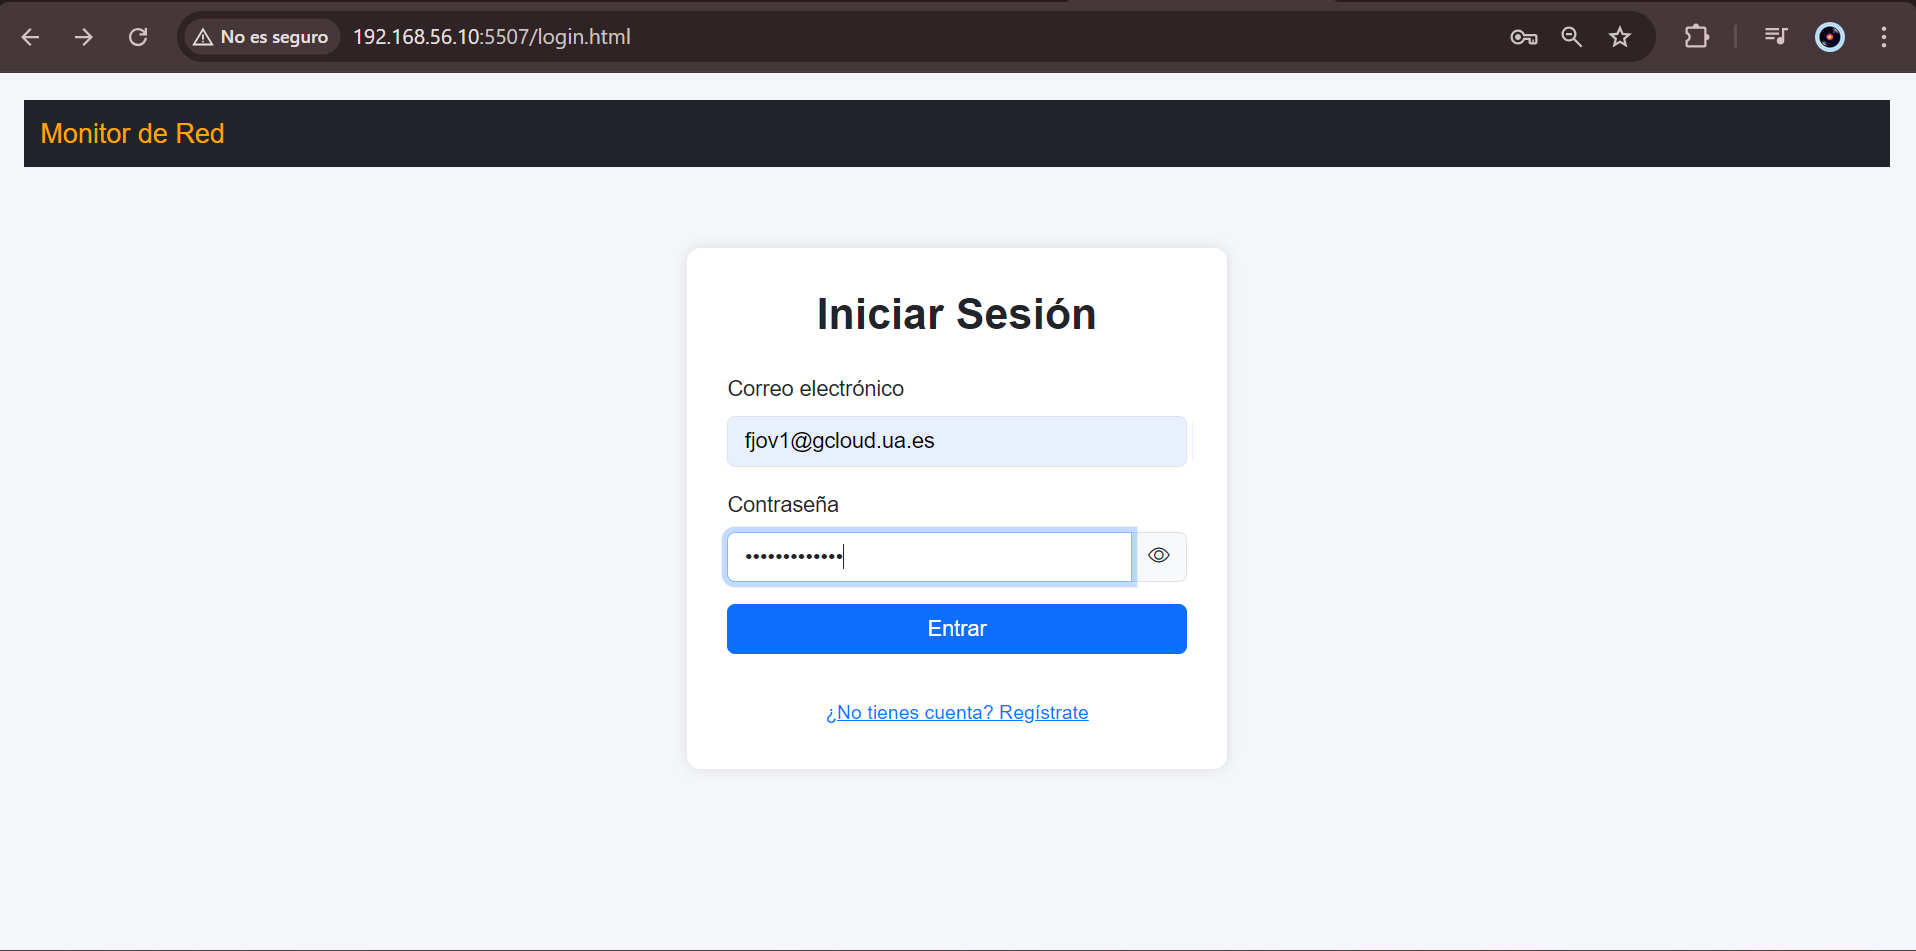
\includegraphics[width=0.7\textwidth]{imagenes/Autenticación.png}
  \caption{Prueba de autenticación de usuario mediante la pantalla de inicio de sesión.}
  \label{fig:prueba-login}
\end{figure}

\subsection{Prueba de monitorización del estado del router}

Una vez autenticado, el usuario puede consultar el estado general de los routers disponibles. Esta prueba verifica la correcta obtención y visualización de información relevante como el \textit{uptime} del dispositivo y el uso de recursos.

El proceso completo implica una solicitud del frontend al backend, la ejecución de comandos del router a través de una conexión SSH y la posterior presentación de los datos en la interfaz web. La Figura~\ref{fig:prueba-estado-router} muestra el resultado de esta prueba, evidenciando el correcto funcionamiento del flujo end-to-end.

\begin{figure}[H]
  \centering
  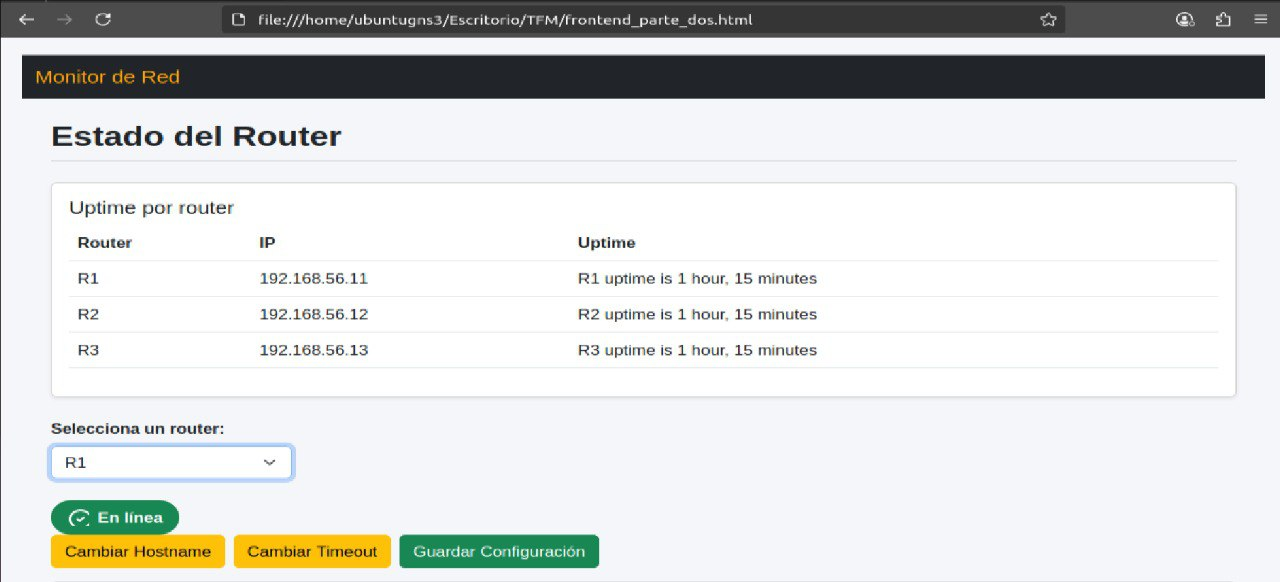
\includegraphics[width=\textwidth]{imagenes/Estado del Router.jpg}
  \caption{Prueba de monitorización del estado del router y visualización de métricas.}
  \label{fig:prueba-estado-router}
\end{figure}

\subsection{Prueba de detección de errores en interfaces}

Con el objetivo de validar el sistema de detección de errores, se forzaron condiciones de error en una de las interfaces del router. El sistema identifica automáticamente la presencia de errores a partir de los contadores obtenidos del dispositivo y los muestra de forma destacada en la interfaz web.

Esta prueba confirma la capacidad del sistema para detectar incidencias de forma automática y presentarlas de manera comprensible para el usuario. En la Figura~\ref{fig:prueba-errores} se pbserva im ejemplo de interfaz con errores detectados correctamente.

\begin{figure}[H]
  \centering
  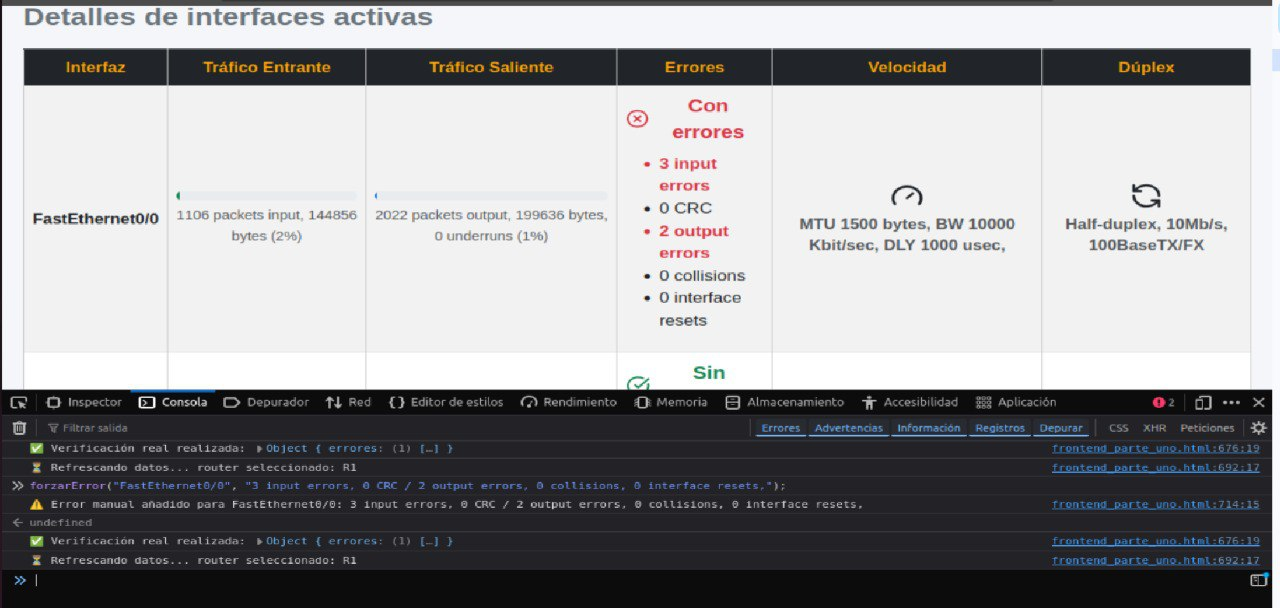
\includegraphics[width=\textwidth]{imagenes/Ejemplo_Errores.jpg}
  \caption{Prueba de detección y visualización de errores en interfaces de red.}
  \label{fig:prueba-errores}
\end{figure}

\subsection{Prueba del sistema de alertas e informes}

Finalmente, se verificó el funcionamiento de alertas mediante la generación automática de un informe cuando se detectan nuevos errores en las interfaces. Ante esta situación, el backend genera un documento en formato PDF con el resumen de las incidencias y los envía por correo electrónico al usuario autenticado.

Esta prueba demuestra la capacidad del sistema para notificar de forma proactiva al administrador de red, añadiendo un valor adicional frente a una simple visualización de datos. En la Figura~\ref{fig:prueba-alerta} se muestra el correo electrónico recibido con el informe adjunto.

\begin{figure}[H]
  \centering
  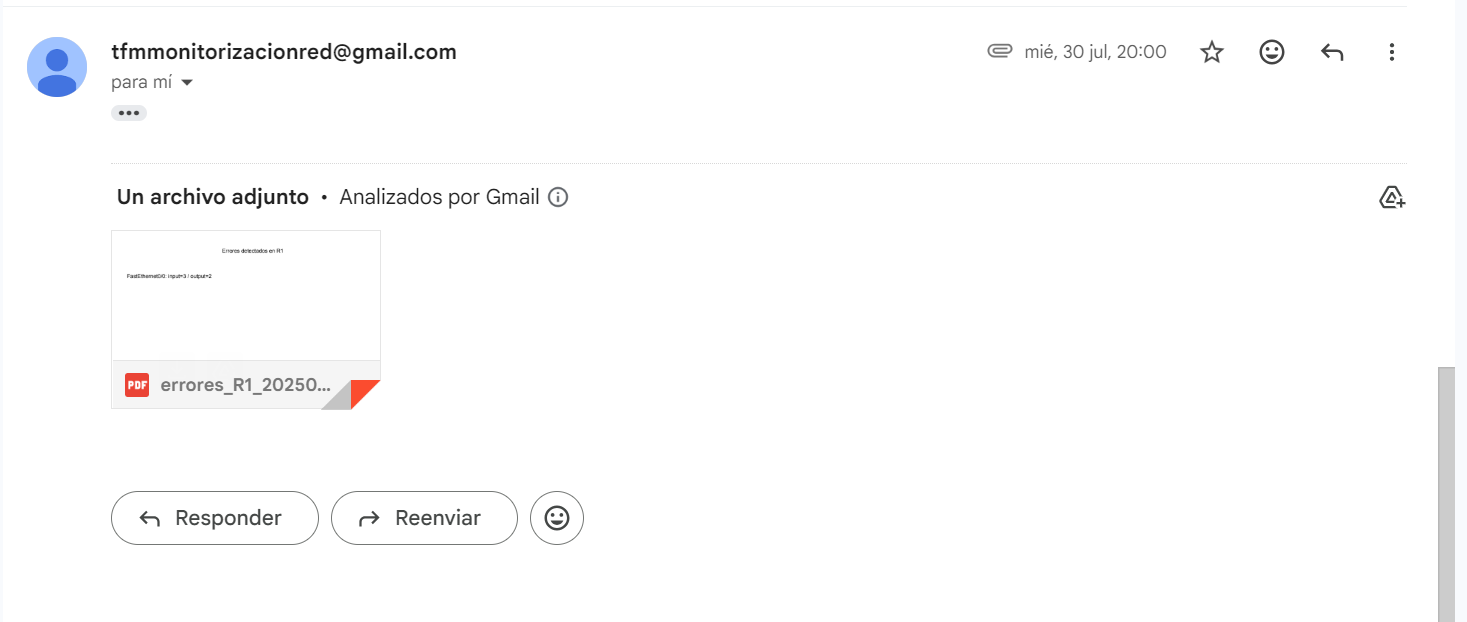
\includegraphics[width=\textwidth]{imagenes/Errores_Correo.png}
  \caption{Prueba del sistema de alertas mediante el envío de un informe por correo electrónico.}
  \label{fig:prueba-alerta}
\end{figure}

\section{Pruebas desde el punto de vista del usuario}

Desde la perspectiva del usuario, el sistema permite acceder de forma sencilla a las distintas funcionalidades de monitorización y gestión mediante una interfaz web intuitiva. Las pruebas realizadas confirman que un usuario autenticado puede navegar entre las diferentes vistas, consultar el estod de los routers, identificar errores y recibir notificaciones sin encontrar bloqueos funcionales.

El flujo de navegación resulta coherente y las acciones disponibles se corresponden con el perfil de usuario de técnico en telecomunciaciones, lo que facilita el uso del sistema inclos para usuario con conocimientos básicos de administración de redes.

